\chapter{Đọc thêm 2: Đòn bẩy và hành vi chấp nhận rủi ro dưới rủi ro đạo đức (Hott)}
\label{ch:M6L4DocThem2}

\section{Thông tin nguồn}

\begin{itemize}
  \item \textbf{Nguồn:} Hott, C. ``Leverage and Risk Taking under Moral Hazard.'' \emph{Journal of Financial Services Research}, 2022.
  \item \textbf{Phần cần đọc:} Chỉ các bảng, hình, biểu đồ và chú thích
  \item \textbf{Ghi chú:} bản chuyển ngữ tiếng Việt súc tích, bám cấu trúc nguồn (giữ nguyên tiêu đề, công thức, số liệu, bảng, chú thích và danh mục tài liệu tham khảo).
\end{itemize}

\begin{figure}[H]
\centering
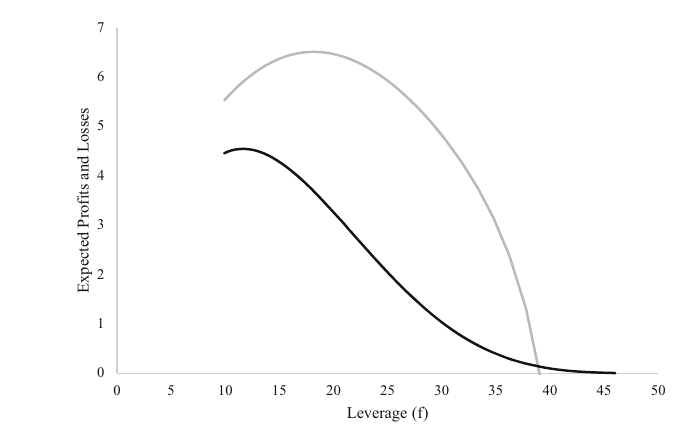
\includegraphics[width=0.85\linewidth]{gfx/m6l4_hott_fig1.png}
\par\smallskip{\small \textbf{Hình 1.} Quan hệ giữa đòn bẩy và lợi nhuận kỳ vọng E(Y) của ngân hàng, cũng như tổn thất kỳ vọng EL của người gửi tiền. P(\ensuremath{\pi}) = 1 \ensuremath{-} \ensuremath{\pi}, I = 50, C = 1 và k(\ensuremath{\pi}) = 0,01/\ensuremath{\pi}. (Nguồn: Hott (2022), Hình 1)}
\end{figure}


Với hai tham số còn lại là C = 1 và I = 50, lợi nhuận đạt cực đại tại \ensuremath{\pi} = 0,21. Hàm chi phí làm cho xác suất vỡ nợ thấp trở nên kém hấp dẫn. Khi chi phí cao hơn, k(\ensuremath{\pi}) = 0,05/\ensuremath{\pi}, xác suất vỡ nợ tối ưu tăng lên 0,23. Đối với các tham số C và I, độ lớn tương đối của chúng quan trọng hơn mức tuyệt đối. Với C = 100

\begin{figure}[H]
\centering
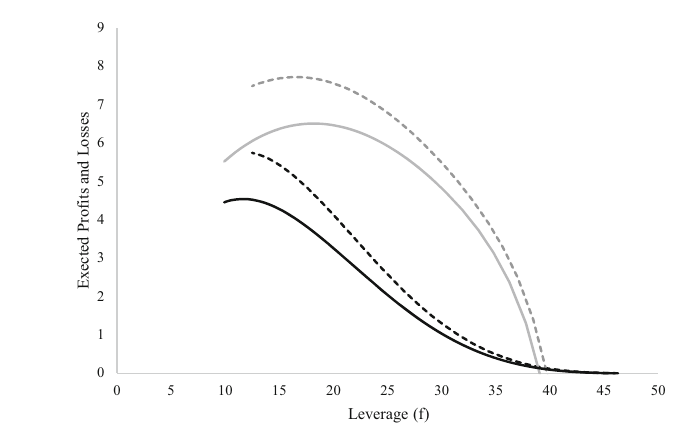
\includegraphics[width=0.85\linewidth]{gfx/m6l4_hott_fig2.png}
\par\smallskip{\small \textbf{Hình 2.} Quan hệ giữa đòn bẩy với tổn thất kỳ vọng (EL và EL\^{}mh) cũng như lợi nhuận kỳ vọng (E(Y) và E(Y\^{}mh)) khi có và không có rủi ro đạo đức. P(\ensuremath{\pi}) = 1 \ensuremath{-} \ensuremath{\pi}, I = 50, C = 1, k(\ensuremath{\pi}) = 0,01/\ensuremath{\pi} và \ensuremath{\beta} = 0,4. (Nguồn: Hott (2022), Hình 2)}
\end{figure}


Khi có bảo lãnh (ngầm định) của chính phủ, tổn thất trực tiếp kỳ vọng của người gửi tiền giảm đi vì chính phủ, với một xác suất nào đó, sẽ chi trả trong trường hợp vỡ nợ. Tuy nhiên, người gửi tiền vẫn chịu tác động gián tiếp vì chính phủ phải tài trợ cho khoản cứu trợ bằng thuế. Do đó, tổn thất kỳ vọng tổng hợp (EL\^{}mh) của người gửi tiền và

\begin{figure}[H]
\centering
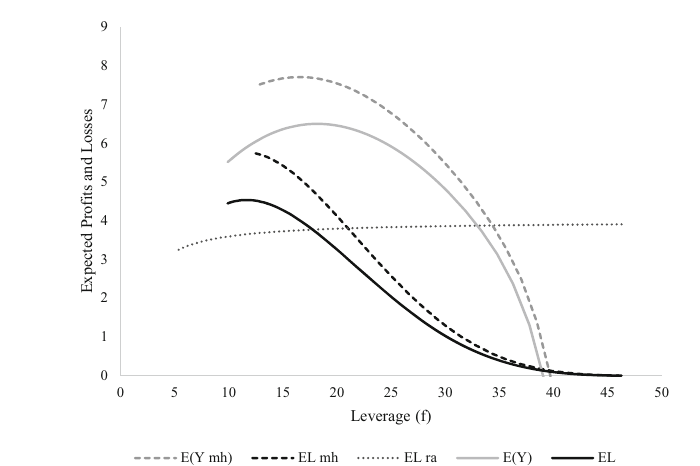
\includegraphics[width=0.85\linewidth]{gfx/m6l4_hott_fig3.png}
\par\smallskip{\small \textbf{Hình 3.} Quan hệ giữa đòn bẩy và các tổn thất kỳ vọng (EL, ELmh và ELra) cũng như lợi nhuận kỳ vọng (E(Y) và E(Y mh)). C = 1, I = 50, \ensuremath{\beta} là 10\%, k(\ensuremath{\pi}) = 0,01/\ensuremath{\pi}, P = 1 \ensuremath{-} \ensuremath{\pi} và \ensuremath{\rho} = 2. (Nguồn: Hott (2022), Hình 3)}
\end{figure}


Các tổn thất tăng đến mức tối đa \ensuremath{\rho}C = 4. Tại đòn bẩy khoảng 18, tổn thất kỳ vọng của ngân hàng hệ thống chịu quy định bằng tổn thất kỳ vọng của chuẩn so sánh (benchmark). Tuy nhiên, đòn bẩy tối đa hóa lợi nhuận khi yêu cầu vốn điều chỉnh theo rủi ro có hiệu lực ràng buộc là khoảng 19 (không hiển thị trong Hình 3).
